\chapter[2022 July]{July 2022}

\section[2022/07/06]{Wednesday, 06 July 2022}

\subsection{Convolution and max pooling algorithms}

The aim of today's session is to implement the convolution and max pooling algorithms and interface them with the basic neural network already implemented. The logic of the convolution algorithm is presented in \FigRef{fig:conv_alg_labbook} and shows how the algorithm will be implemented from first principles. \\

\begin{figure}[h]
    \centering
    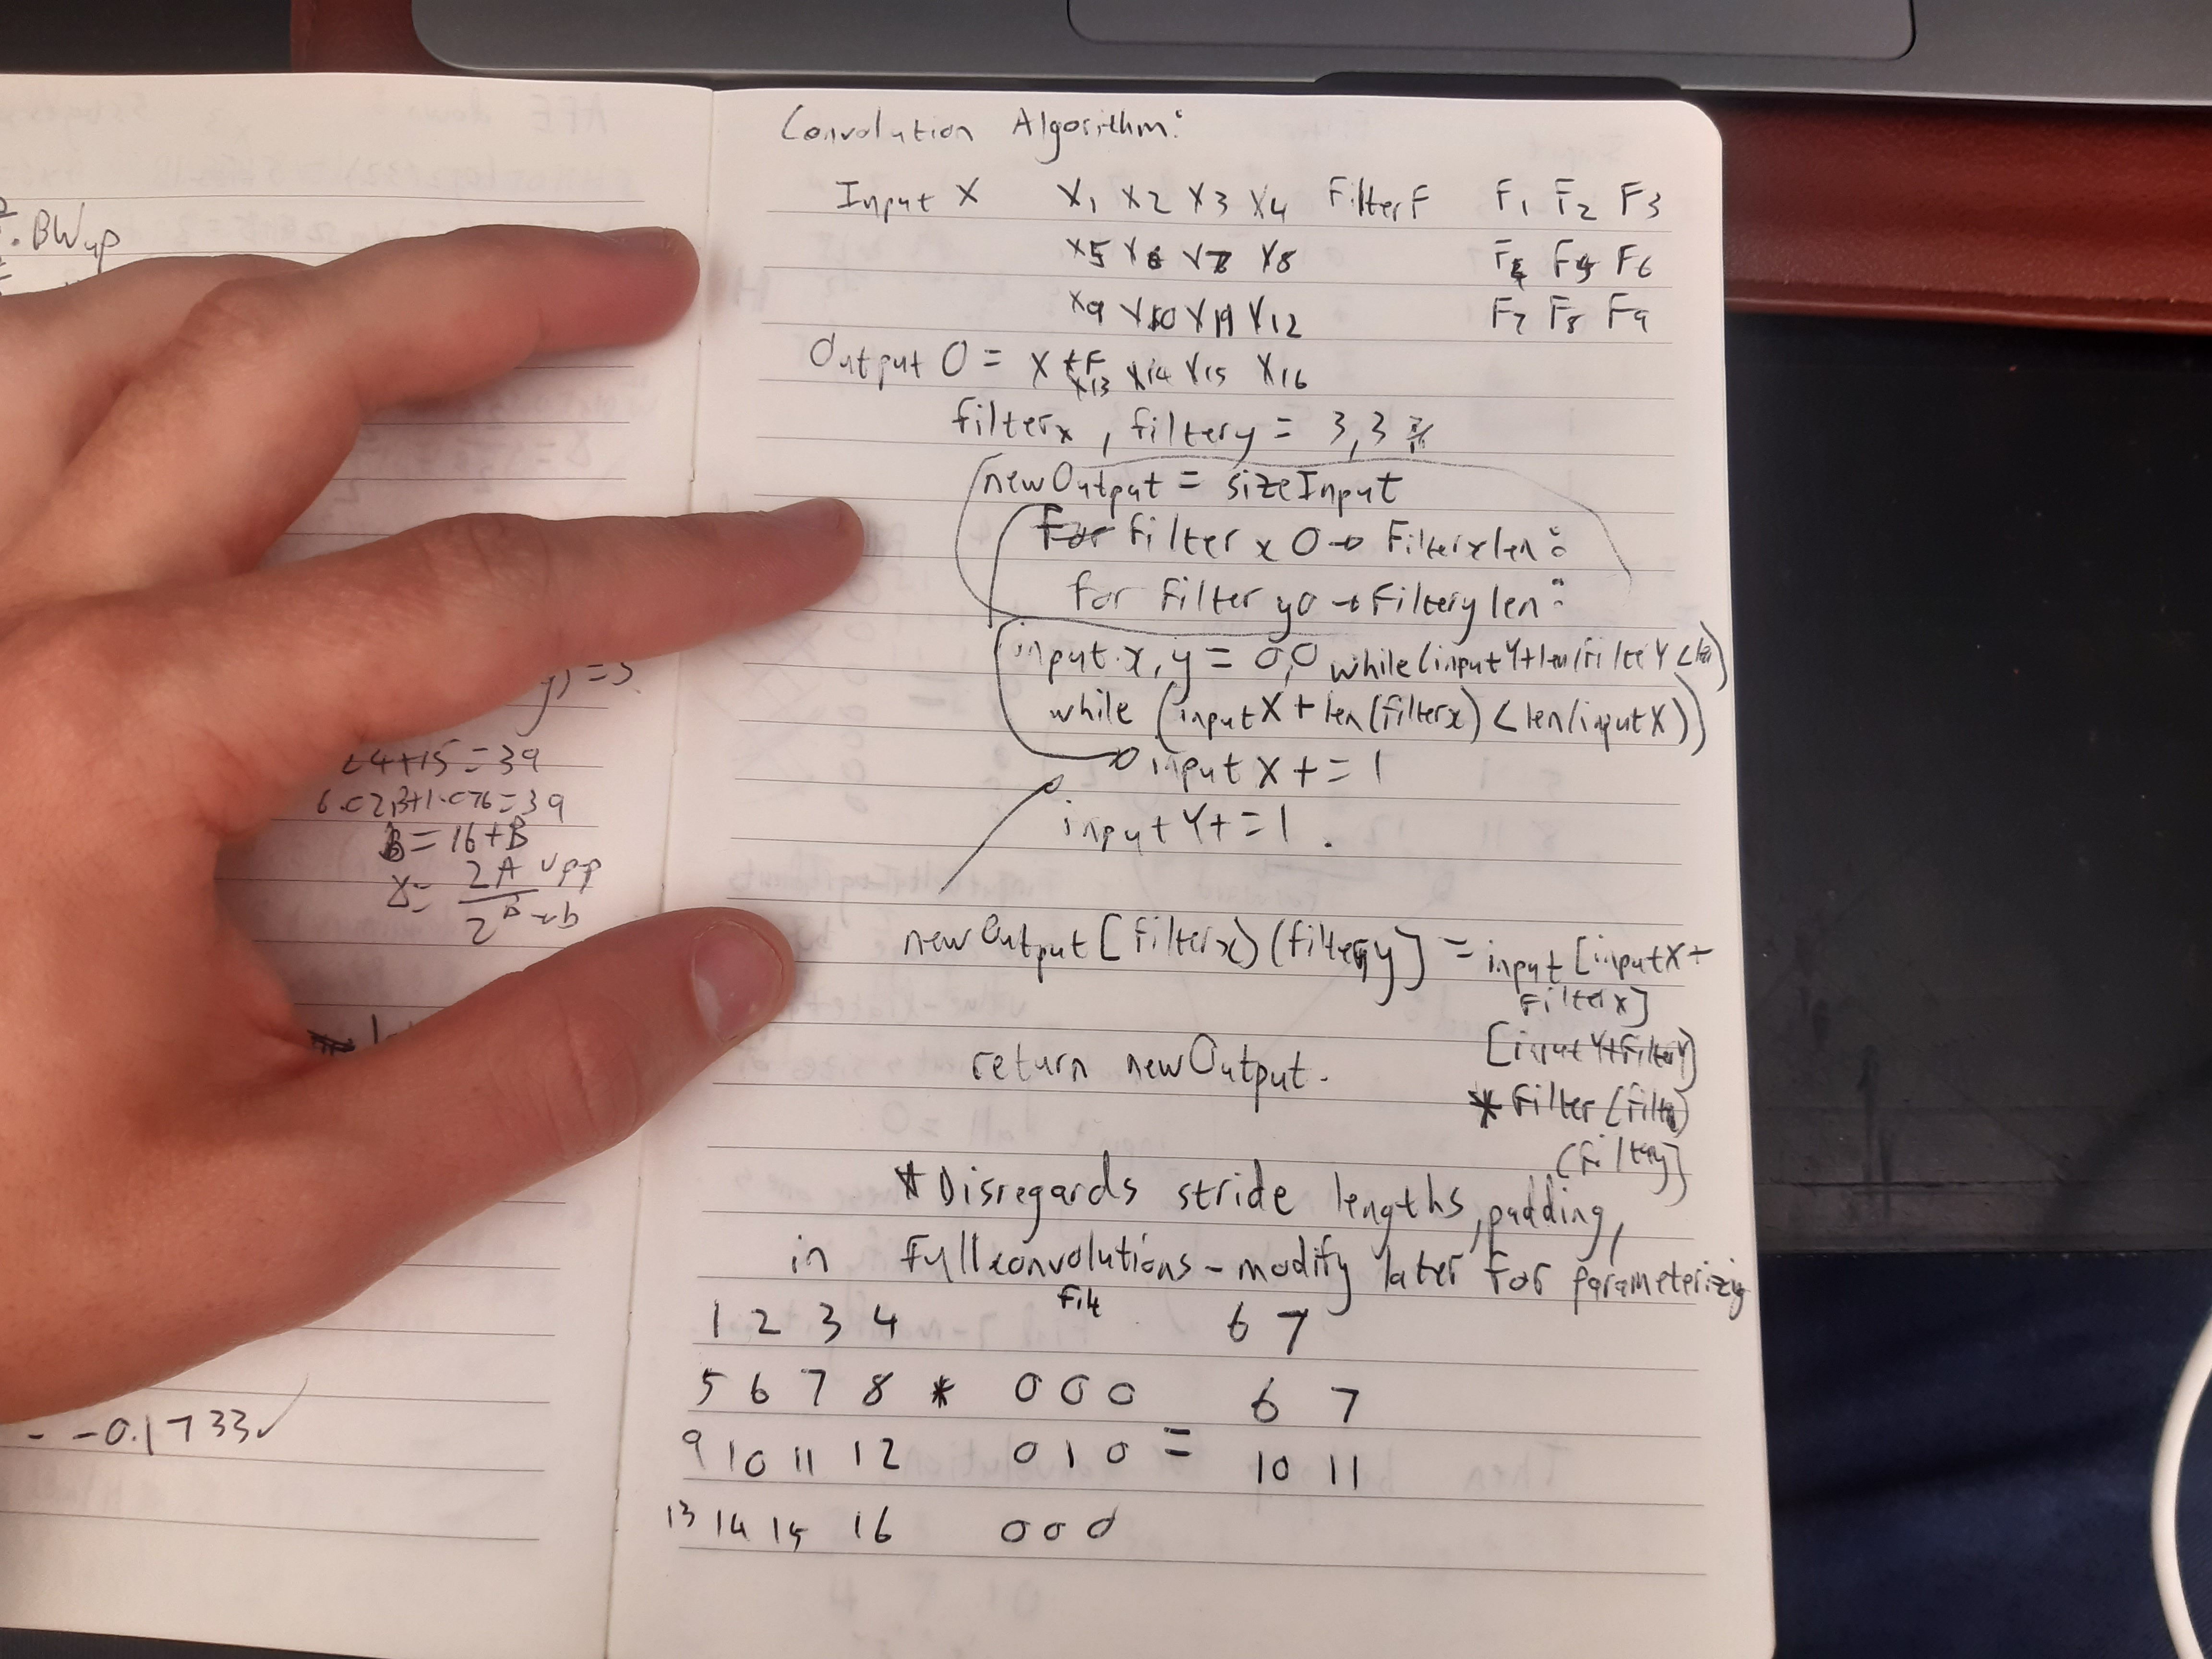
\includegraphics[width=1.0\linewidth]{figures/conv_alg_labbook.jpg}
    \caption{Proposed logic for convolution algorithm}
    \label{fig:conv_alg_labbook}
\end{figure}

The convolution algorithm is initially constructed with stride length one and zero padding and accepts an input and filter matrix. A counter iterates over the entire input matrix and another counter sums all the multiplications between the current portion of the input matrix and each element of the filter. This sum is then placed into the first position in an output matrix. The intuition and calculations described here were first evolved from the calculations shown in \FigRef{fig:conv_maths_labbook}.

\begin{figure}[h]
    \centering
    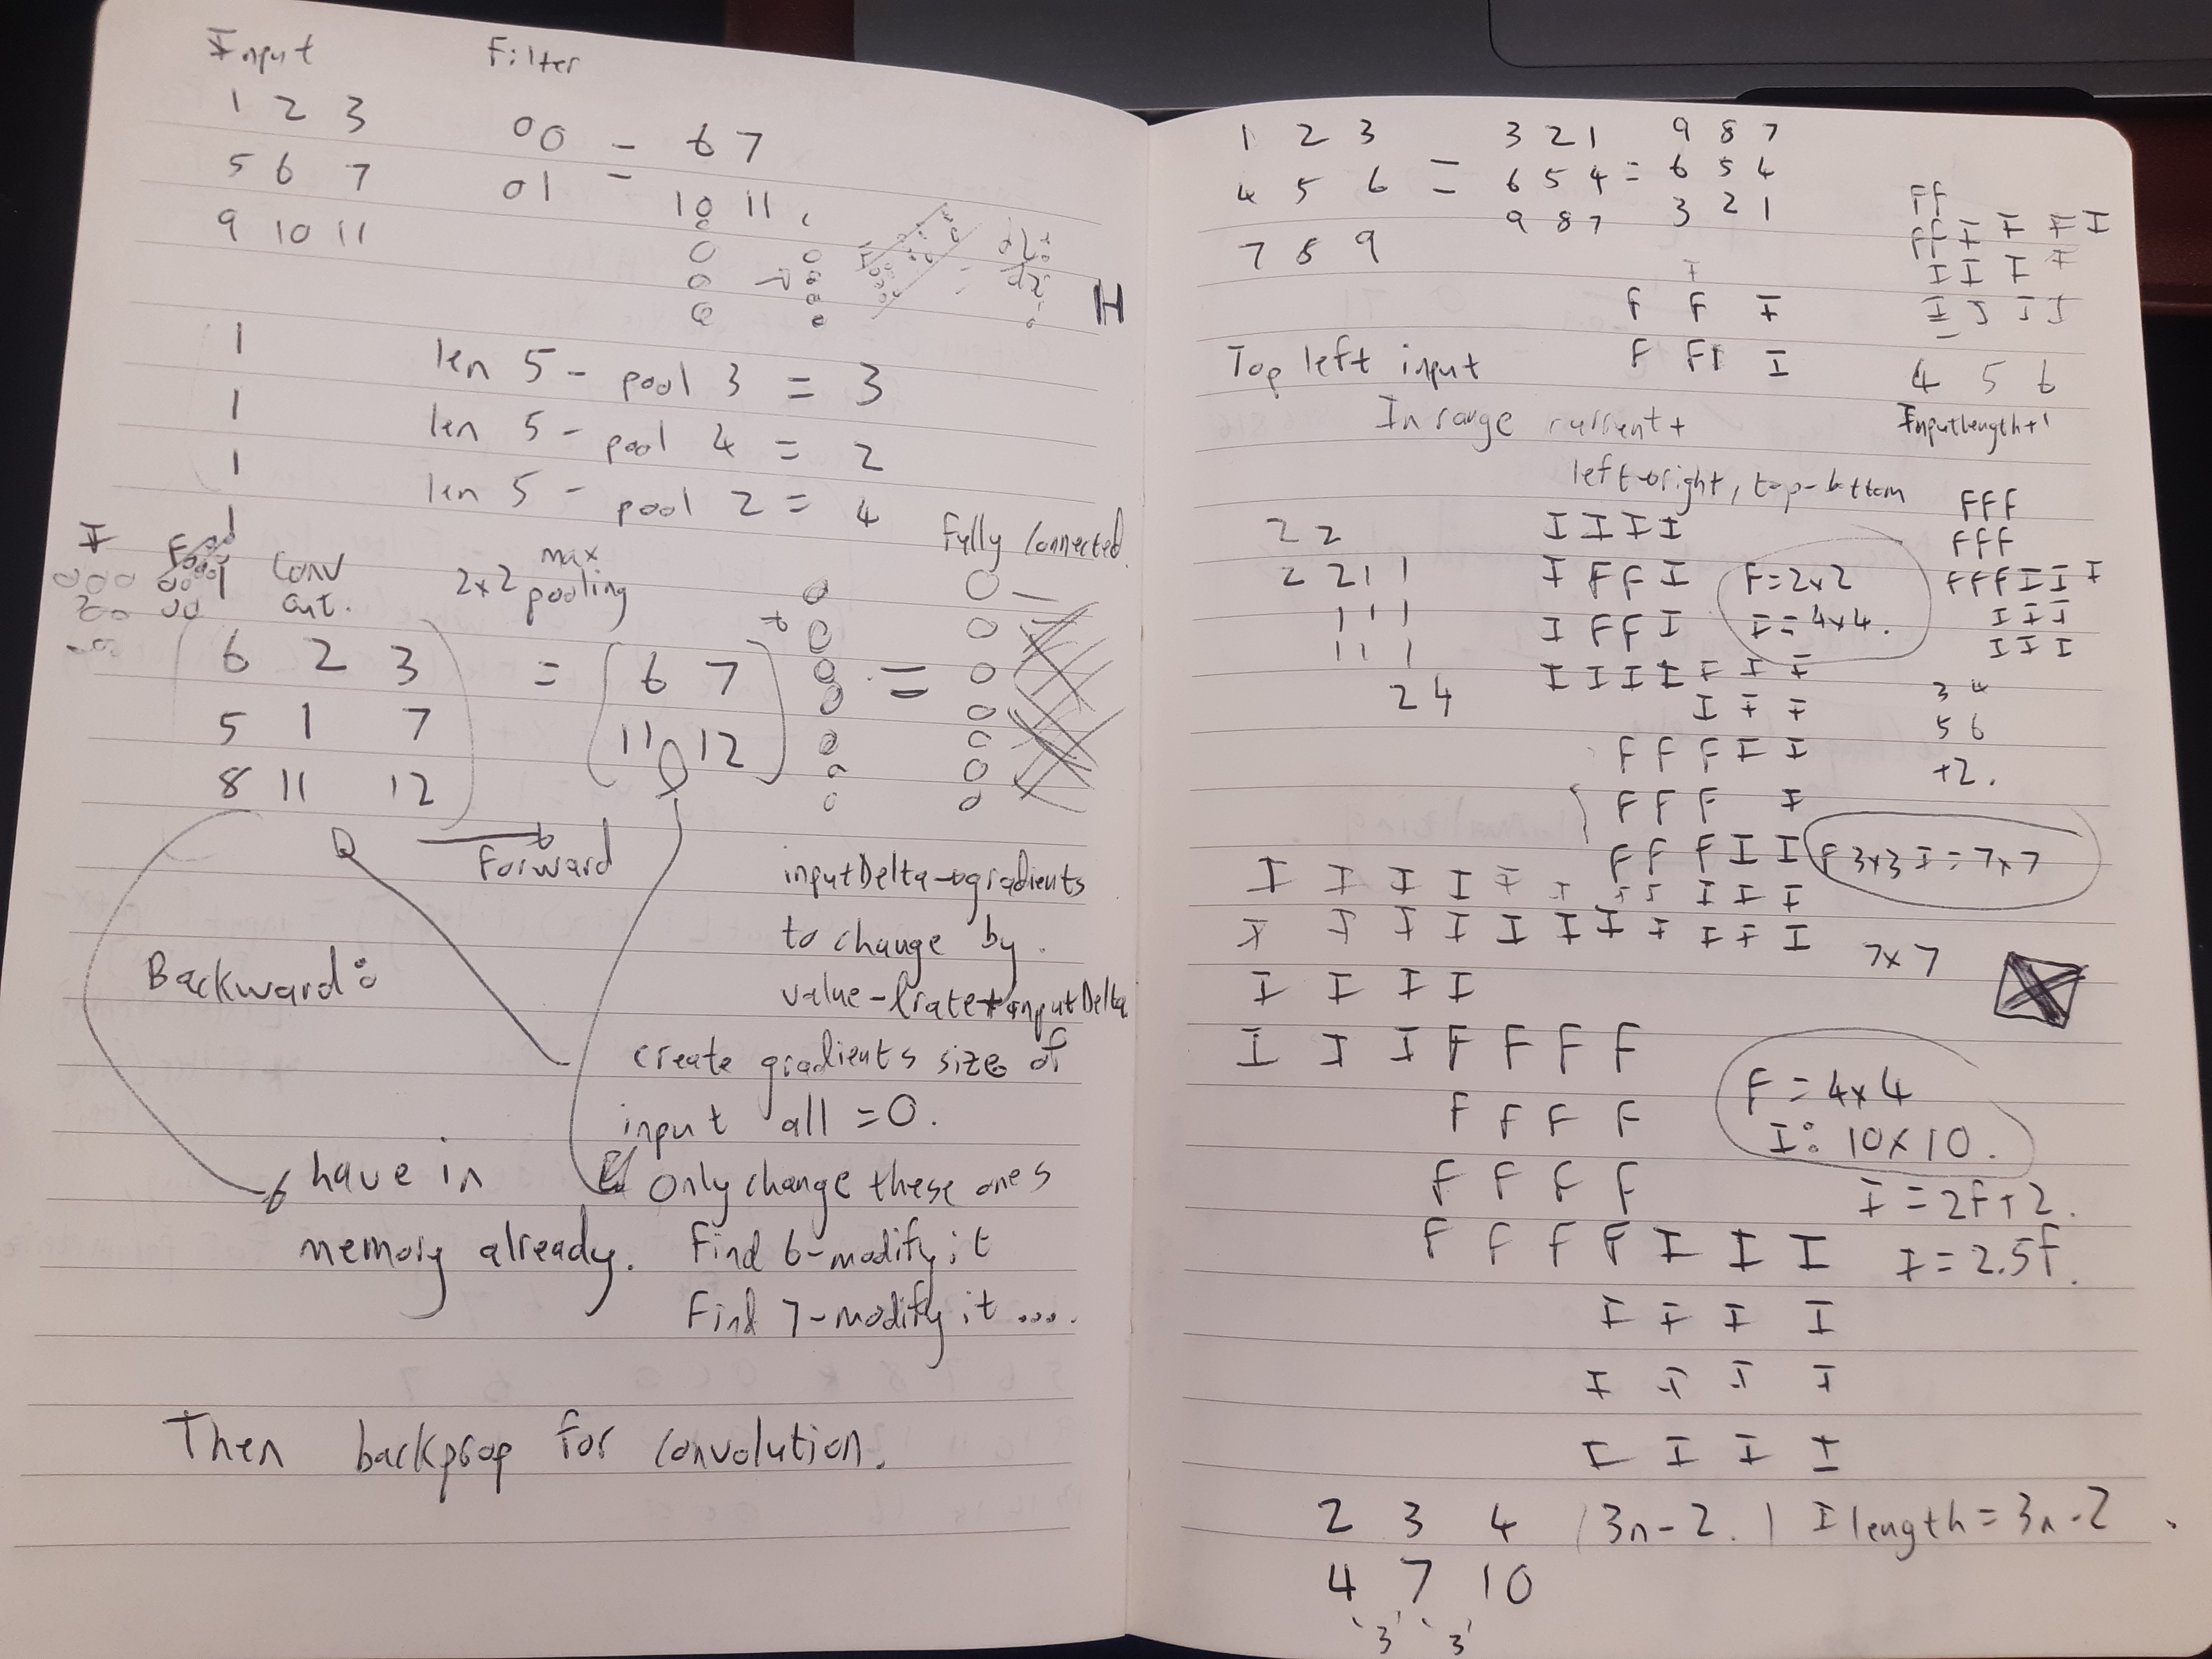
\includegraphics[width=1.0\linewidth]{figures/conv_maths_labbook.jpg}
    \caption{Calculations and logic for convolution algorithm}
    \label{fig:conv_maths_labbook}
\end{figure}

The max pooling algorithm has a modifiable pool length and stride length and accepts an array of neurons that represents the layer of the network to be max pooled. Similarly to the convolution algorithm, a counter iterates over the entire previous layer and considers each pool-length by pool-length portion of the previous layer and finds the maximum value in this portion of the matrix. This maximum value is placed in an output matrix.

\section[2022/07/07]{Thursday, 07 July 2022}

\subsection{CNN backpropogation for convolutional layers}

Further work was conducted today on the max pooling algorithm and implementing the backpropagation of the convolutional layers - this involved finding the gradient of each filter element based on the error backpropogated from the fully-connected neural network to the max-pooling layer. The max-pooled output is found inside the convolutional layer and the gradient applied to this specific part of the filter by performing the convolution of the input image data and the error from the previous layer. 

\section[2022/07/08]{Friday, 08 July 2022}

\subsection{Basic CNN testing}

A single image was inputted into the convolutional neural network today in order to establish that the network could overfit and that the backpropagation process was working correctly. The backpropagation algorithm was also modified so that it did not crash upon running - this was due to incorrectly-shaped hidden and output layer gradients being created.

\section[2022/07/12]{Tuesday, 12 July 2022}

\subsection{Troubleshooting exploding weights and saturating neurons}

The past several days were spent troubleshooting the neural network and trying to establish why the weights of the network were getting larger and larger and why all the neurons in both the hidden layer and output layer were all saturating at a value of 1.0. After printing out all of the values of the neurons in each layer it was realized that the sigmoid activation function was outputting the 1 value for all its inputs because the initial input to the network was not normalized and was just the RGB value of each pixel ranging from 0-255. After normalizing the input by dividing by 255 so a value between 0 and 1 was presented as input the problem seemed to be mostly rectified. Further modifying the initial values of the weights to be randomly set to between -1 and 1 improved the network training a lot and prevented the saturation of all neurons in the hidden and output layers. The learning rate was changed to 0.001 from 0.1 and although the network took much longer to train the loss of the network improved a lot - down from around 8 to 0.01 for one input image. \\

Successfully overfitting one image was the initial goal of building the network and the work session today went far towards achieving that goal. Furthermore, the sigmoid activation function was swapped out for a relu activation function but the exploding weights and saturating neurons value became an issue again - further troubleshooting of the forward propogation process might be necessary since the industry standard for activation functions in convolutional neural networks working with images is the relu function. Normalizing the output of each neuron before activation might be a necessary step. Another parameter that needs to be tweaked in future is the stride length used in the convolution operation - how far along the input matrix to move the filter matrix for each multiplication in the convolution operation. The mathematics of the convolution operation however have proven difficult to get right and troubleshoot so this is left for a future work session.

\section[2022/07/13]{Wednesday, 13 July 2022}

\subsection{Output debugging in a textfile}

The aim of the work session today was to enable better output debugging of the network. To that end, a writeToTextFile method was created that could accept strings and integers and then output those values to a textfile in the same directory as the network that was erased and updated every time the network was run. This enabled the full visualization of all the neurons in the hidden and output layer as well as what the values of the filters are - thus making it possible to identify that the filters were not changing as they should be - the problem being that with only one input image the value of the filter did not really need to change as the fully connected neural network was changing enough to reduce the loss at the output of the network. Adding more training images rectified this problem. Additionally, the full convolution required in the backpropagation of the convolutional layers was implemented using the scipy convolution2d method to be replaced by a first principles implementation in future. 

\section[2022/07/14]{Thursday, 14 July 2022}

\subsection{MNIST hand-written digit classifier}

The aim of the work session today is to modify the convolutional neural network in order to create a MNIST hand-written digit classifier just to confirm that the network can learn and predict image values correctly. Ten input images were downscaled to 28x28 and fed into the network. The output layer was modified to only have 10 output neurons while the hidden layer has 1000 neurons and the network was trained over 300 epochs - enough to get the loss down below 1.0. \FigRef{fig:mnist_first_5_results} shows the output of the first five input images to the MNISt classifier which are images of the handwritten digits 0-4. The output shows that the largest value (highest probability) in each test case is the correct value - the first neuron for the input image showing a 0 and the second neuron for the input image showing a 1. To make it easier to understand the output, the final layer of the network should be a softmax layer which just outputs the number neuron with the highest probability in the output layer. Thus the CNN can classify handwritten 28x28 digits.\\

\begin{figure}[h]
    \centering
    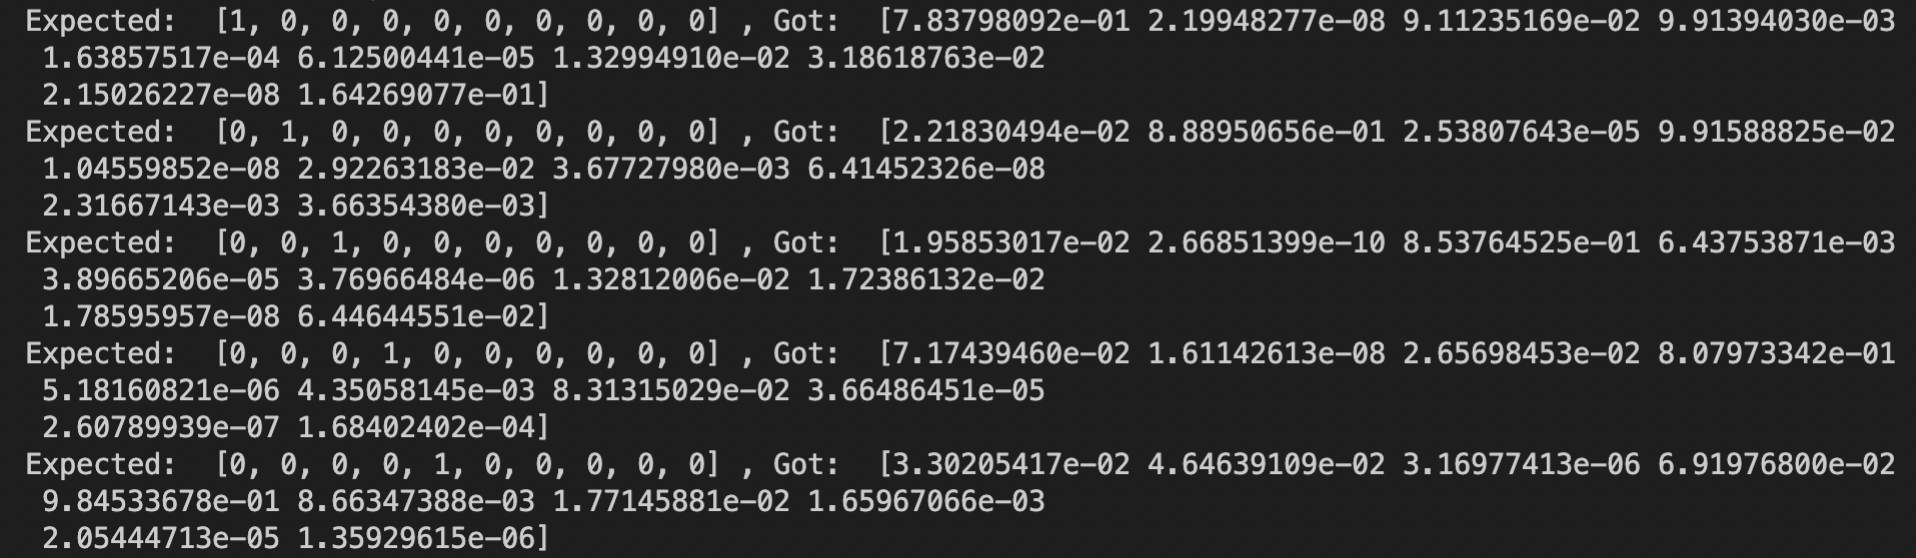
\includegraphics[width=0.8\linewidth]{figures/mnist_first_5_results.png}
    \caption{First five output results of the MNIST classifier}
    \label{fig:mnist_first_5_results}
\end{figure}

The network however took over 6 seconds to run each epoch and as a testing scenario lead to the concern about the network not being optimized enough for realtime use - especially later when the network will need to predict hand positions over 24 times a second. Thus it is going to be necessary to optimize the network, rewrite the convolutional operation as well as optimize processes like the max pooling if the network is going to perform adequately at a later date.  \\

It is noted too that the revised project proposal was received from Prof. Hanekom today and the proposal was accepted. The accepted proposal has been placed in the proposal folder in the project repo and now stands as the standard with which to measure progress and the project's capabilities against.

\section[2022/07/16]{Saturday, 16 July 2022}

\subsection{Single hand coordinate classifier}

Time was spent the previous two work sessions on saving the weights of the CNN to a .npy file for easy re-use and to enable "trained" networks to be used again without having to repeat the whole training process everytime the network was initialized. The MNIST classifier was modified to instead attempt to predict the location of a single hand coordinate when given an input image of a hand. The principle design decision with regards to this was whether to make the output layer a collection of neurons that represented the prescence of a hand landmark at a specific pixel (thumbInPixel1,thumbInPixel2...) or to have the output layer a collection of neurons that represented the normalized xy coordinate value of each hand landmark (thumbXPosition,thumbYPosition,pinkyXPosition...) The proposed architecture for the hand coordinate convolutional neural network architecture is presented in \FigRef{fig:hand_conv_arch_labbook}. \\


\begin{figure}[h]
    \centering
    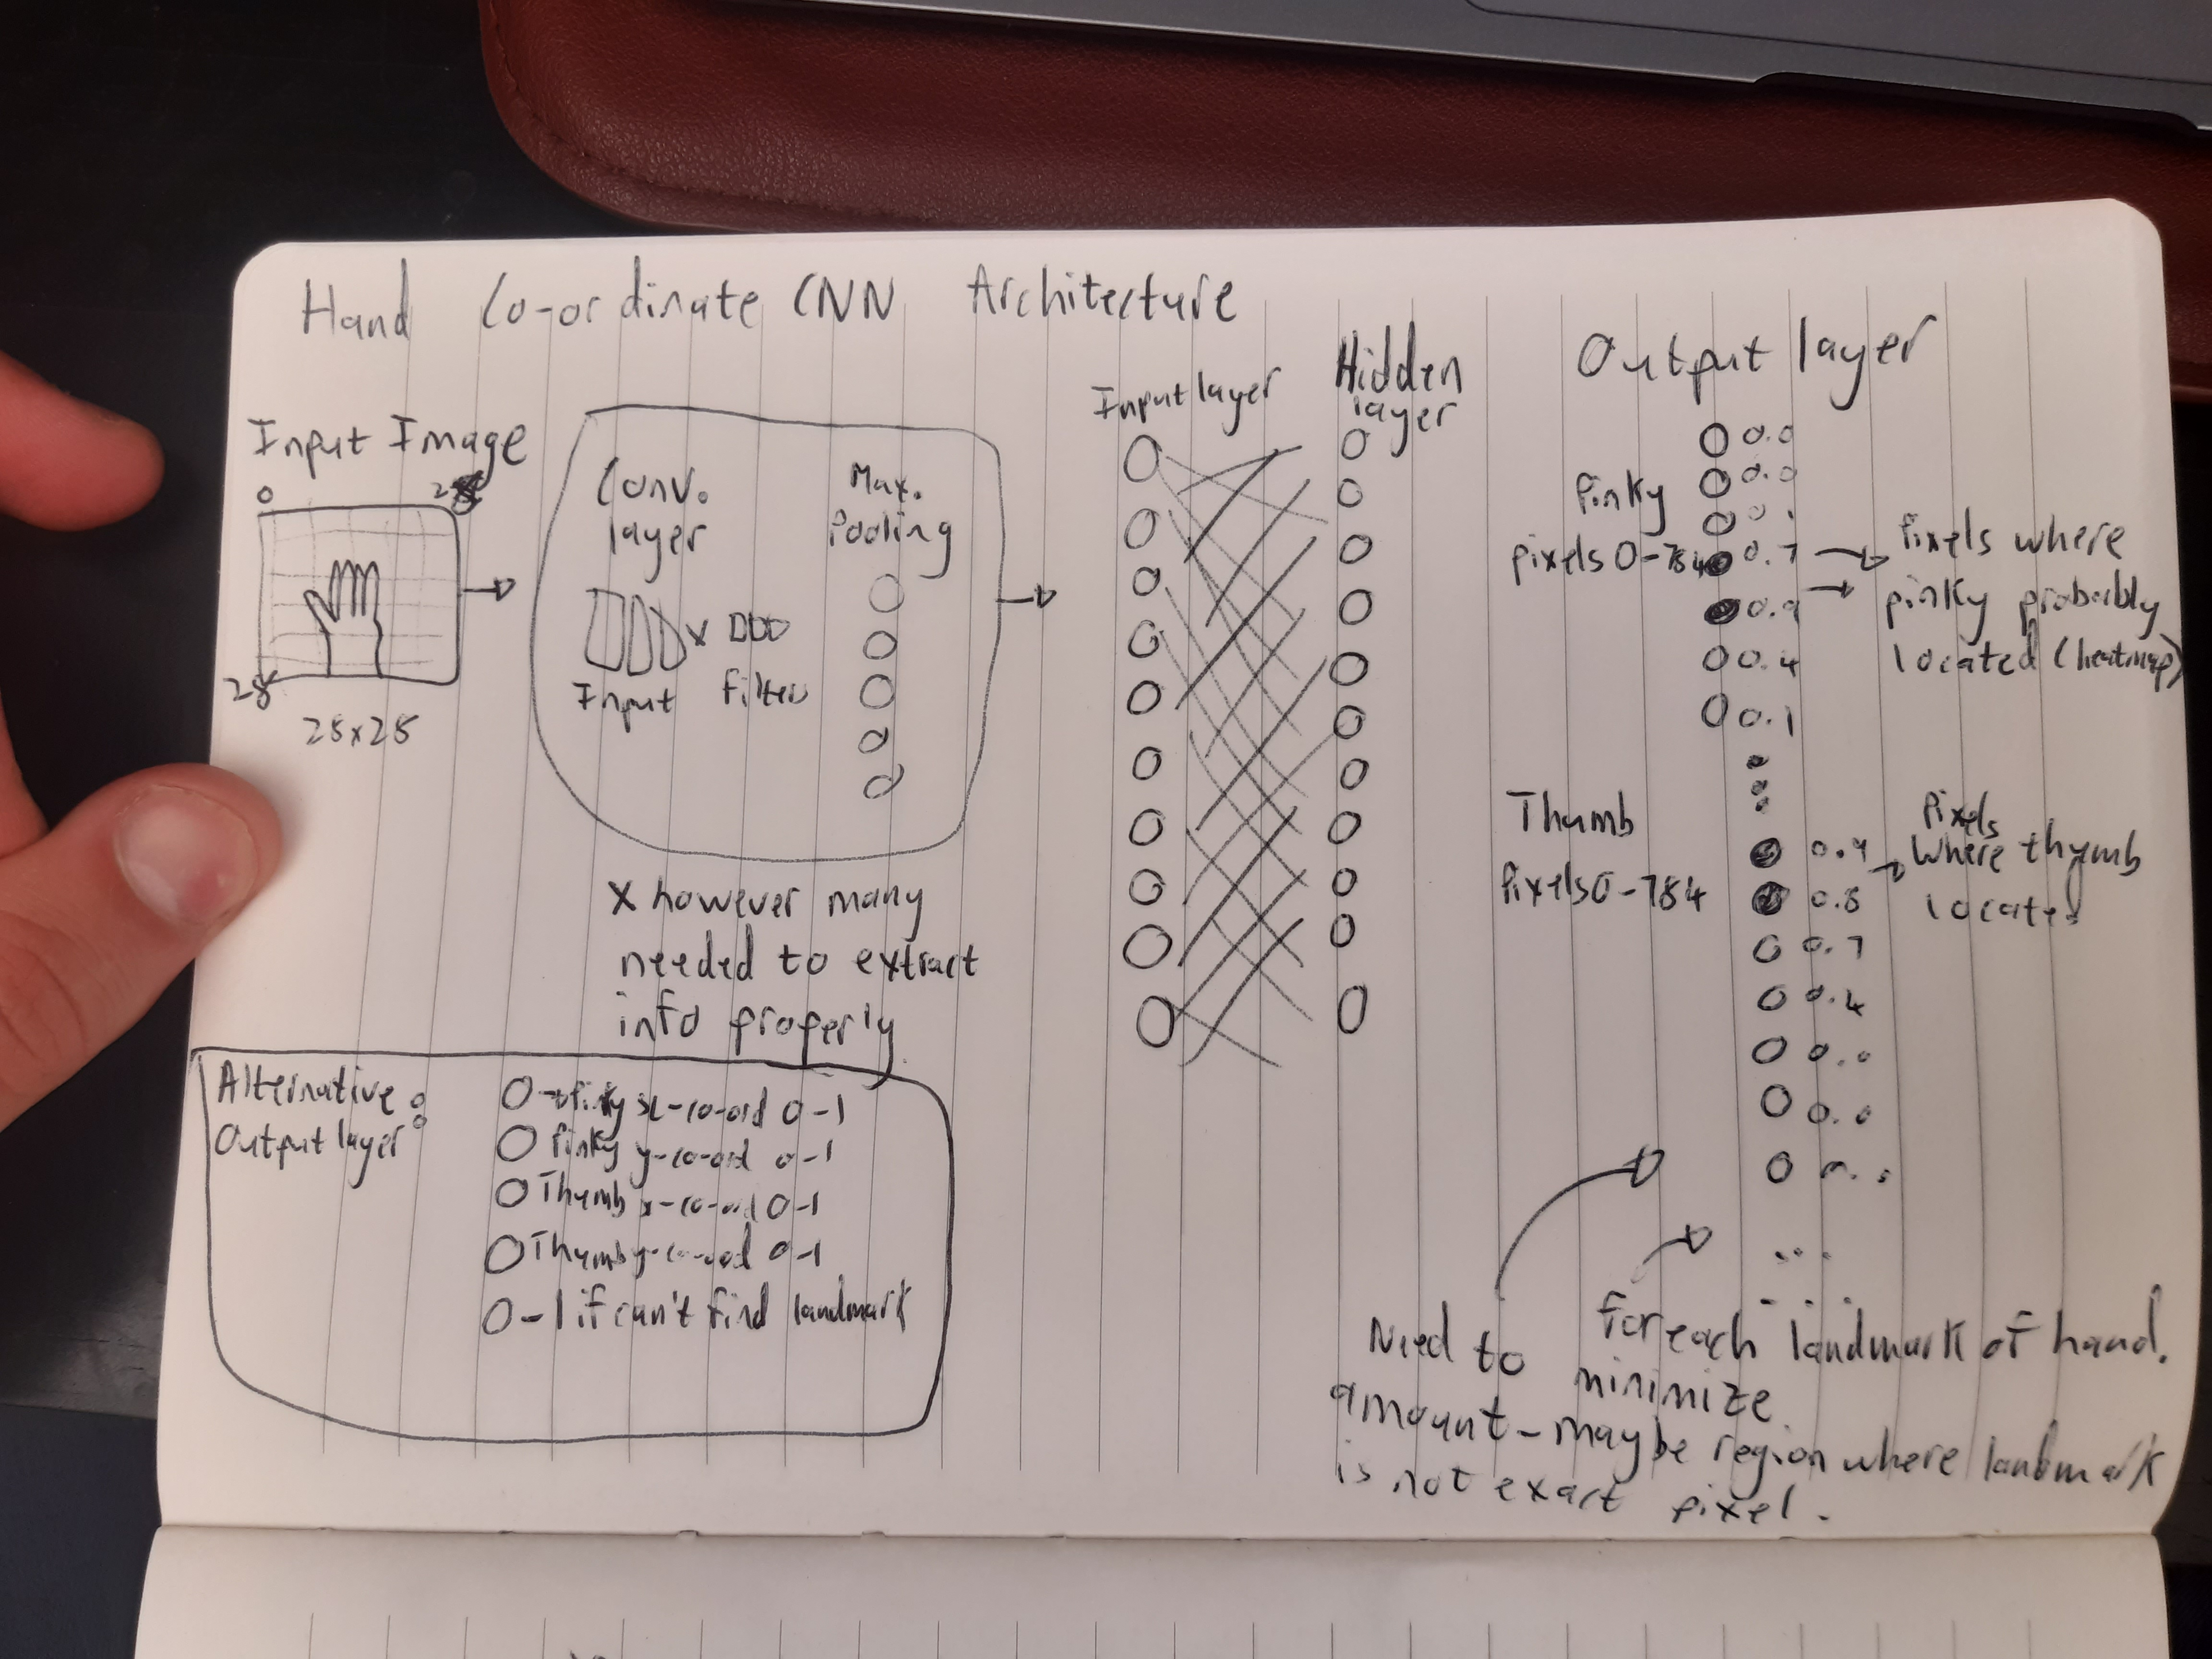
\includegraphics[width=1.0\linewidth]{figures/hand_conv_arch_labbook.jpg}
    \caption{Proposed architecture for hand coordinate convolutional neural network}
    \label{fig:hand_conv_arch_labbook}
\end{figure}

The second option was the first to be attempted because it is so much less memory intensive and the coordinates were set up from 0-1 for both the x and y dimension starting at the bottom left of the input image. The loss of the network was very high and did not seem to be able to classify a single digit. It was postulated that the use of only a single convolutional and max pooling layer was not enough to extract meaningful information from the input image. Thus time was spent adding a second convolutional and max pooling layer. This work was continued on the 18th of July when the backpropagation method was modified to account for the new convolutional layer.

\section[2022/07/19]{Monday, 19 July 2022}

\subsection{Gesture classifier}

The aim of today's work session is to build a system that can accept hand landmark coordinates and predict the gesture that is represented by those coordinates of the hand.

This system will be implemented with a neural network that takes in 42 input parameters (the x and y coordinates of 21 hand landmarks) and output 9 nine numbers that represent the probability that the hand coordinates represent the nine gestures: "one", "two", "three", "four", "five", "fist", "peace", "rock on" and "okay." These gestures were decided upon to maximize the difference between their physical representations and because the natural "up" and "down" gestures of pointing a finger up or down is easily misinterpreted by the network if the image is merely flipped upside down. 1 hidden layer with 100 neurons is used and the network is trained on 45 input images (5 images for each gesture). \\

The loss curve for the learning process is presented below in \FigRef{fig:gesture_recognizer_loss_curve}. Some examples of the system accurately classifying gestures are presented in the figures below. The system used mediapipe hands to provide the hand landmark coordinates to the gesture classifier as this has not been accurately completed from first principles yet. The system however does not function excellently and when the hand gesture is presented in different orientations the system cannot classify it properly. This can be remedied with more training data showing the gestures in various orientations and a higher number of neurons in the hidden layer. This will be attempted at a later date when higher accuracy is required.

\begin{figure}[h]
    \centering
    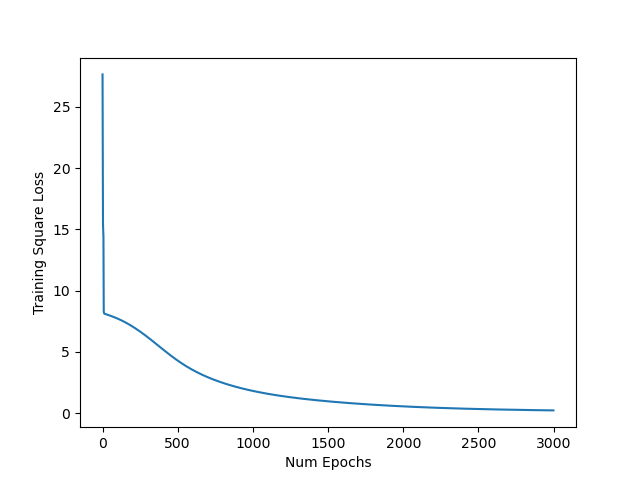
\includegraphics[width=0.6\linewidth]{figures/gesture_recognizer_loss_curve.png}
    \caption{Loss curve of the gesture recognition neural network}
    \label{fig:gesture_recognizer_loss_curve}
\end{figure}

\begin{figure}[h]
    \centering
    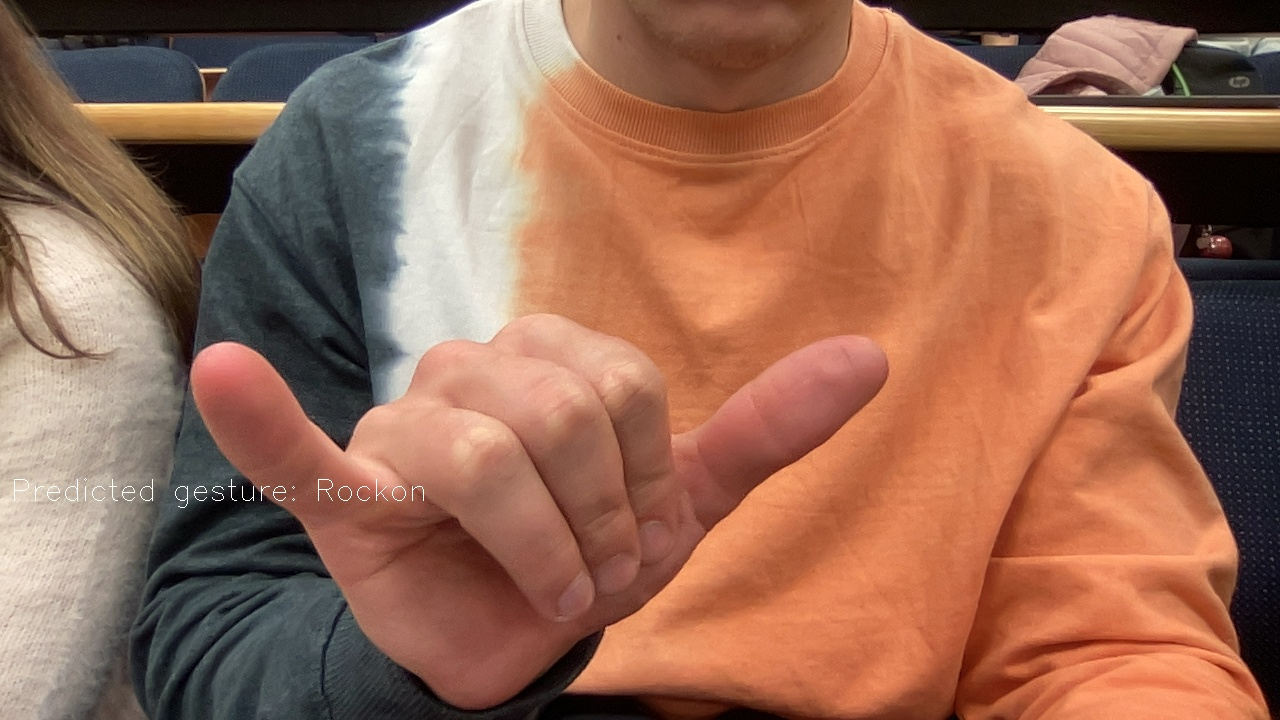
\includegraphics[width=0.6\linewidth]{figures/predictedGesture_rockon.jpg}
    \caption{Predicted gesture using gesture recognition neural network}
    \label{fig:predictedGesture_rockon.png}
\end{figure}

\begin{figure}[h]
    \centering
    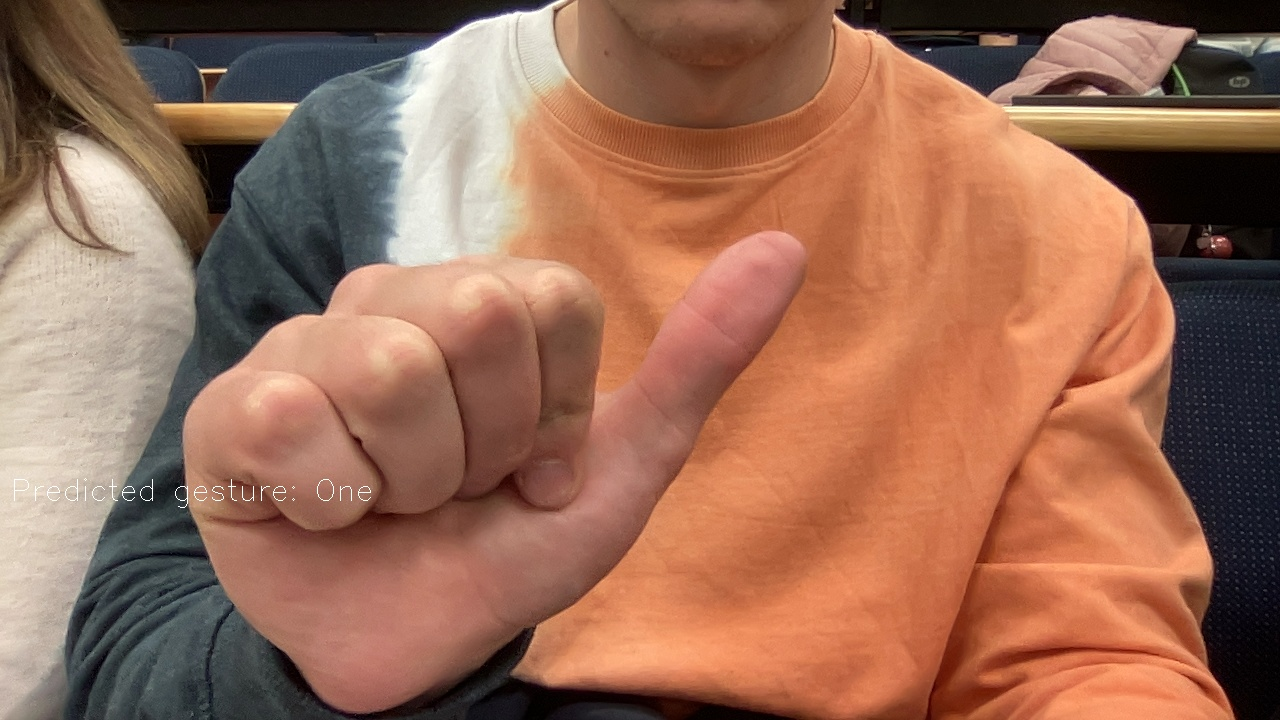
\includegraphics[width=0.6\linewidth]{figures/predictedGesture_one.jpg}
    \caption{Predicted gesture using gesture recognition neural network}
    \label{fig:predictedGesture_one}
\end{figure}

\begin{figure}[h]
    \centering
    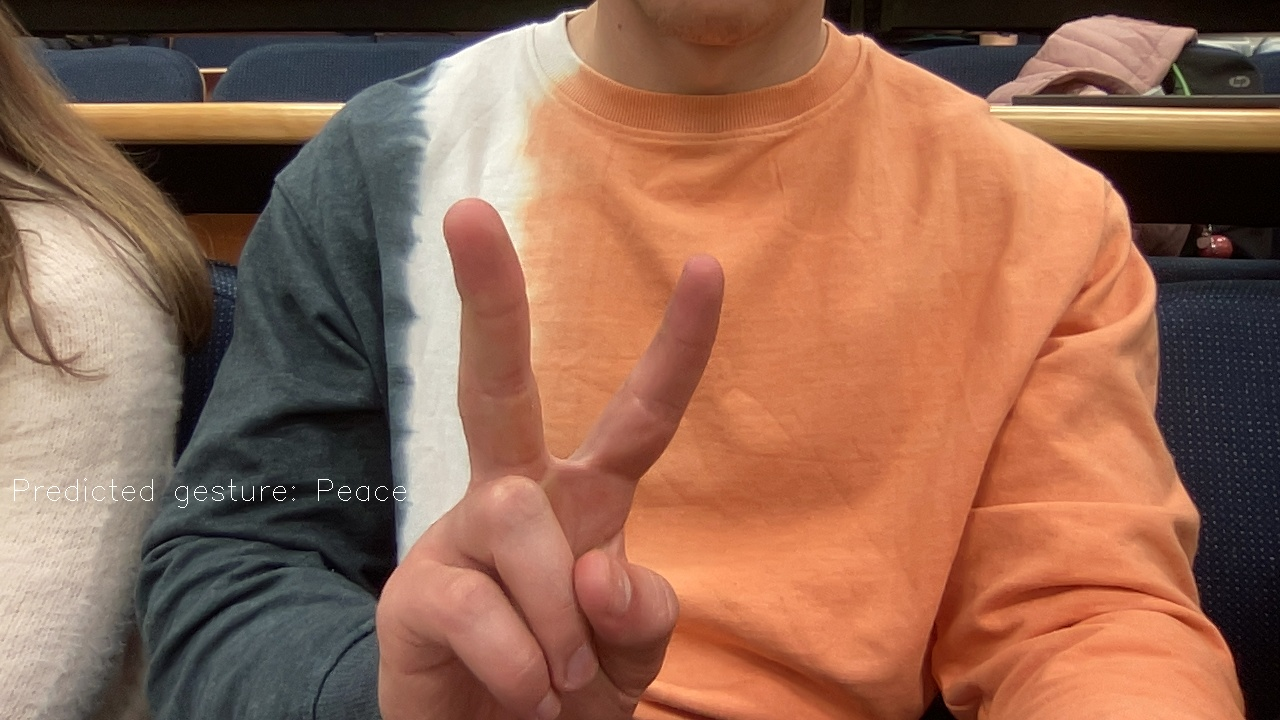
\includegraphics[width=0.6\linewidth]{figures/predictedGesture_peace.jpg}
    \caption{Predicted gesture using gesture recognition neural network}
    \label{fig:predictedGesture_peace}
\end{figure}

\begin{figure}[h]
    \centering
    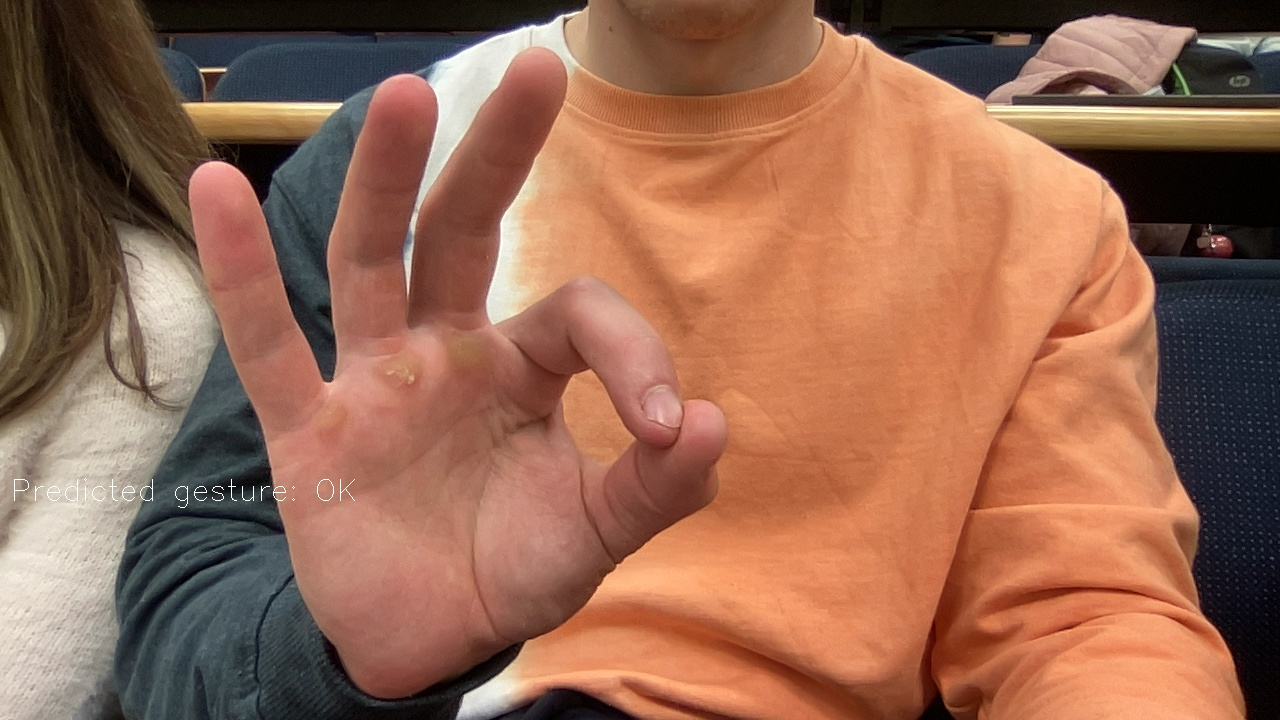
\includegraphics[width=0.6\linewidth]{figures/predictedGesture_ok.jpg}
    \caption{Predicted gesture using gesture recognition neural network}
    \label{fig:predictedGesture_ok}
\end{figure}

\section[2022/07/25]{Monday, 25 July 2022}

\subsection{Kinect camera edge detection}

The aim of today's work session is to experiment with convolving the images from the Kinect camera with various filters in order to detect edges of objects presented to the camera - in aid of detecting objects to be interacted with in augmented reality by the virtual object.\\

A prototype was constructed to take the input of the Kinect camera and convolve it with a modified edge detection filter so that only the outlines of shapes and objects in the camera feed are visible in the output of the program. The result is displayed in \FigRef{fig:kinect_filter_edges}. This method fails to take advantage of the Kinect depth information however and only shows the edges of objects in two dimensions, not three - thus an alternative approach using the depth data needs to be devised to find the edges of objects in three dimensions. Perhaps a combination of the depth data at a relevant edge pixel will be able to inform an algorithm if an object can be moved through that particular coordinate in virtual space.

\begin{figure}[h]
    \centering
    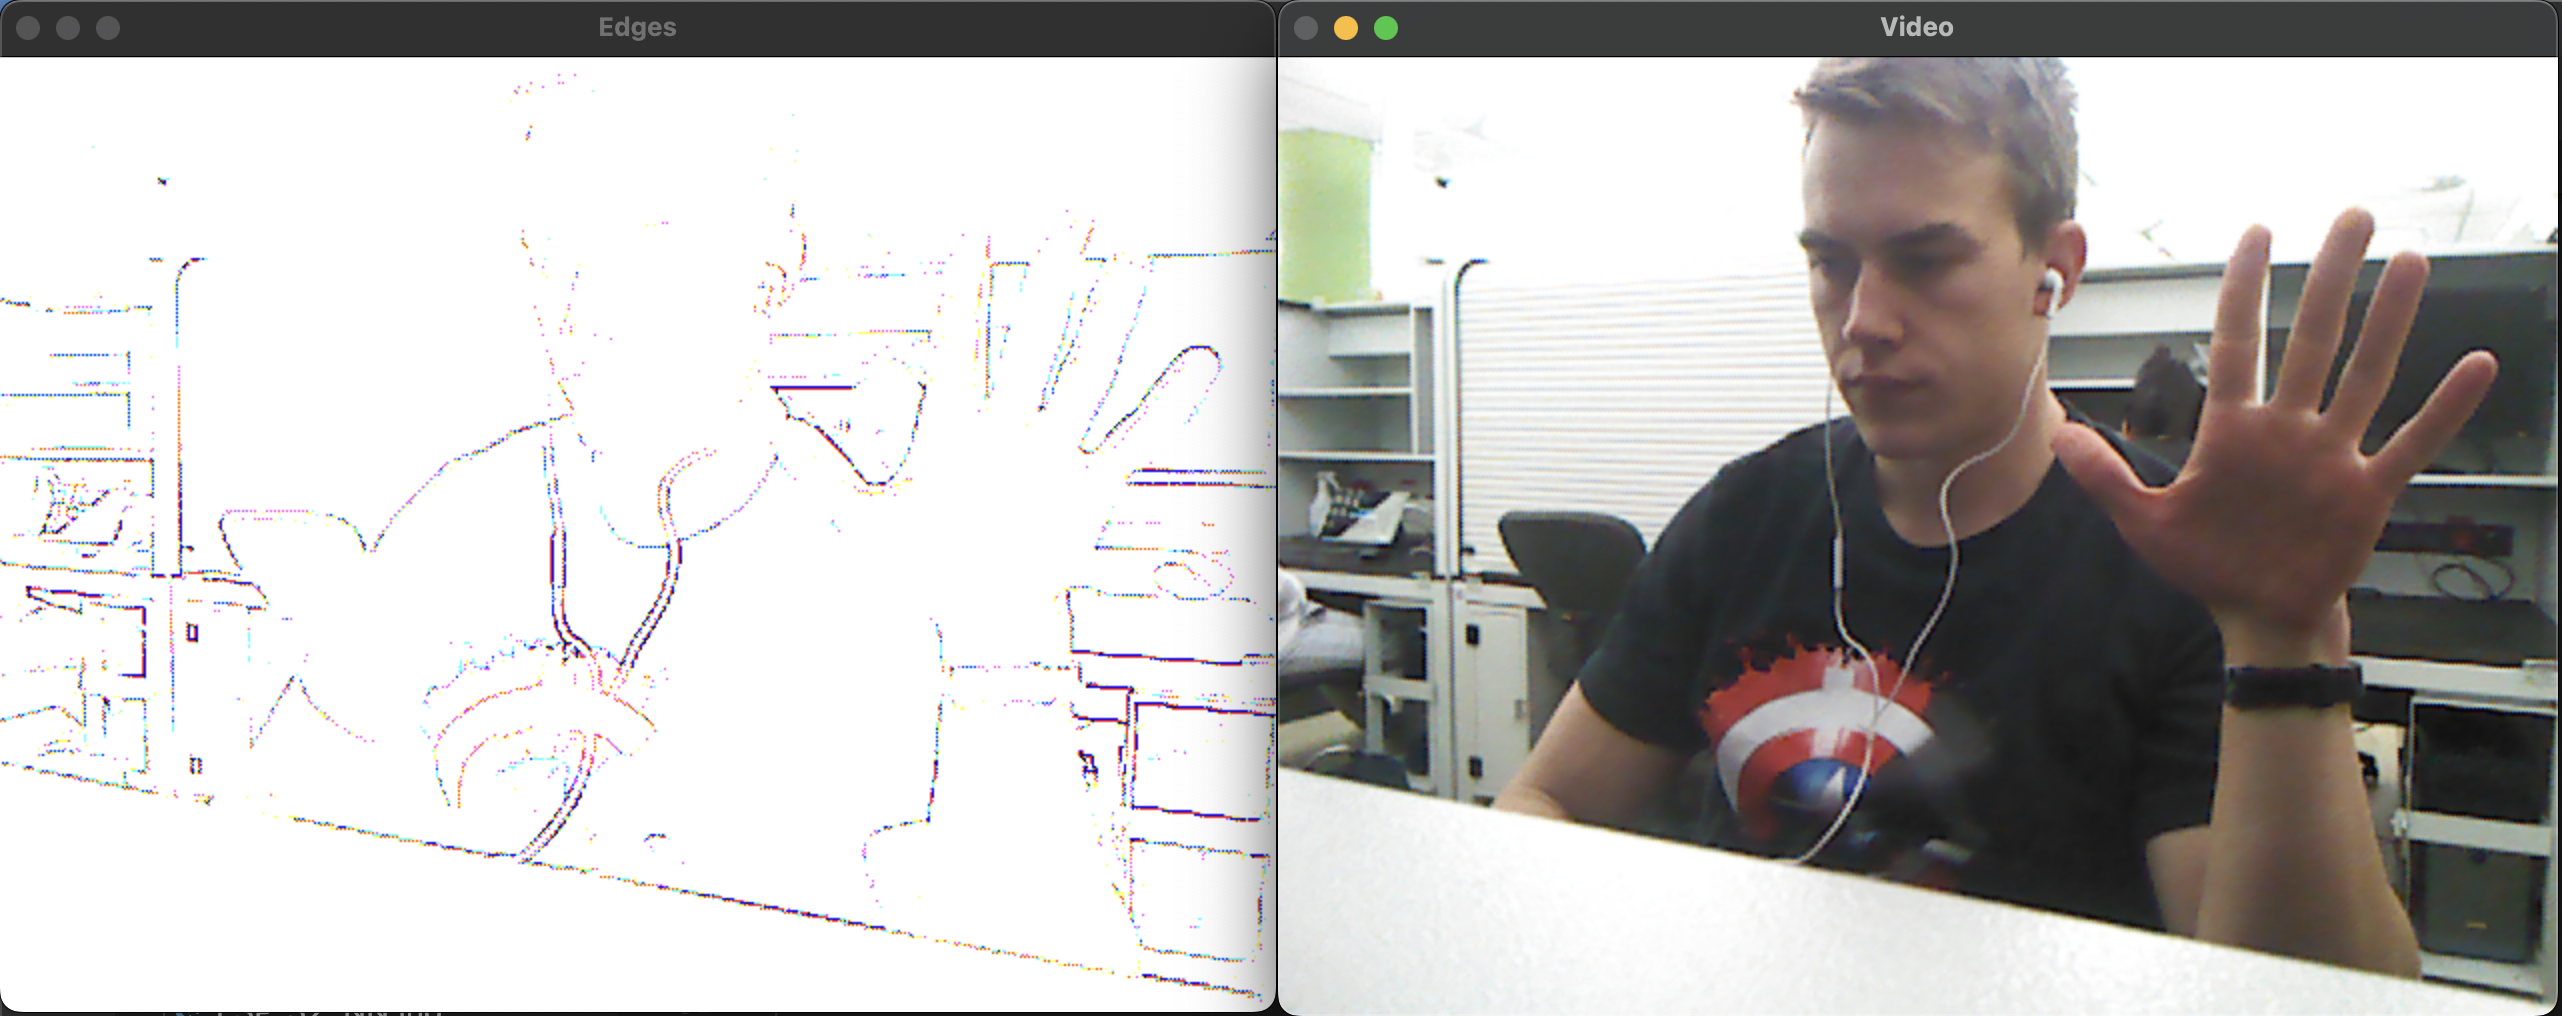
\includegraphics[width=0.9\linewidth]{figures/kinect_filter_edges.png}
    \caption{Output of convolution of Kinect imagery with modified edge detection filter}
    \label{fig:kinect_filter_edges}
\end{figure}

It is hypothesized that the final implementation of a collision avoidance algorithm will need to have the following attributes in order to complete its function of integrating the virtual object with the real environment:

\begin{itemize}
  \item Each xyz pixel in the virtual space must either be an edge or non-edge of an object
  \item Depth data at each pixel must be available to determine how far back that object issue
  \item The virtual object must also have xyz coordinates
  \item The virtual object xyz coordinates must be checked against the environment's xyz coordinates to prevent collisions
\end{itemize}

It is noted that the depth output from the Kinect camera is an integer value from 0-2048 where 2048 represents a depth value closest to the camera and 0 a value far away from the camera. This can be taken advantage of in order to display the different values using a colormap to represent depth. The results of this process is visible in \FigRef{fig:kinect_colormap}. Thus in order to conduct collision avoidance a three-dimensional coordinate system can be created that is x=camera width, y=camera height and z=0-2048 depth dimensions large and a set of coordinates using this same scale that maps the virtual object's position in the environment to the coordinate system outlined here. A conversion algorithm will have to be created in order to map the coordinate system's position of the virtual object into OpenGL coordinates for rendering. It is also going to be necessary to shrink the apparent size of the cube as it is moved around the screen in order to create perspective and the illusion of augmented reality.

\begin{figure}[h]
    \centering
    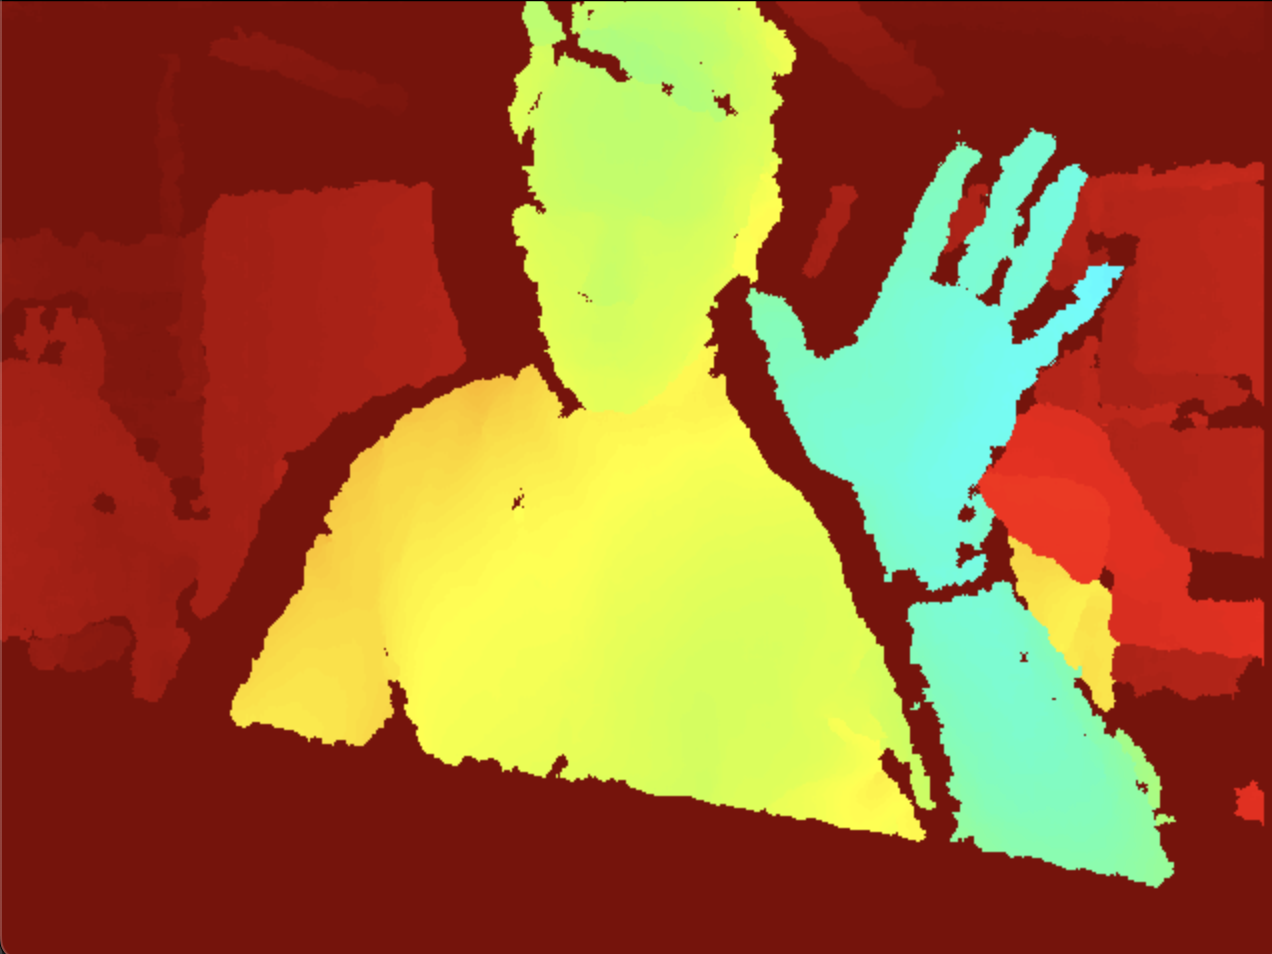
\includegraphics[width=0.6\linewidth]{figures/kinect_colormap.png}
    \caption{JET colormap interpretation of Kinect depth data}
    \label{fig:kinect_colormap}
\end{figure}

A large amount of time today was also spent converting the neural network architecture developed so far into a more modifiable and expandable format using classes and methods - this will enable layers to be added and removed far more easily and will increase readability and understanding of the network. As of the end of the work session, this has mostly been accomplished save for the backwards propagation of the various layer types and forward propagation of the convolutional and maxpooling layers.

\section[2022/07/26]{Tuesday, 26 July 2022}

\subsection{Neural network refactoring }

The aim of the work session today is to continue refactoring the convolutional neural network code for better testing and expansion. After many hours of examining convolutional neural network theory, the network was optimized to allow multiple filters to be used in each convolutional layer - a feature that had been overlooked in the previous implementation and has now been rectified. The use of several convolutional layers in succession however is still non-functional due to the layer being coded to only accept input images with three channels - not multidimensional arrays which are the output of previous convolutional layers. This problem was worked on for many days after this work session and served as a major source of frustration.

